\documentclass{article}

    \usepackage[utf8]{inputenc}
    \usepackage[T1]{fontenc}
    \usepackage{aeguill}
    % \usepackage[francais]{babel}
    \usepackage[a4paper]{geometry}
    \usepackage{array}
    \usepackage{amsfonts}
    \usepackage{amsmath} 
    \usepackage{amssymb}
    \usepackage{amsthm}
    \usepackage{xspace}
    \usepackage{dsfont}
    \usepackage{collcell}
    \usepackage{datatool}
    \usepackage{enumitem}
    \usepackage{xstring}
    \usepackage{booktabs}
    \usepackage{environ}
    \usepackage{bbm}
    \usepackage{hyperref}
    \usepackage{graphicx}
    \usepackage{caption}
    \usepackage{stmaryrd}
    \usepackage[dvipsnames]{xcolor}
    \usepackage{tikz}
    \usetikzlibrary{trees}
    \usepackage{ulem}
    \usepackage{cancel}
    \usepackage{pgfplots}
    % \usepackage{minted}
    % \usemintedstyle{monokai}
    \usepackage{multicol}
    
    \pgfplotsset{compat=newest}
    \usetikzlibrary{automata} % LATEX and plain TEX
    \usetikzlibrary[automata] % ConTEXt
    \usetikzlibrary{arrows}
    \usetikzlibrary{automata,arrows,positioning,calc}
    \xdefinecolor{vertf}{named}{OliveGreen}
    \xdefinecolor{rougef}{named}{BrickRed}
    \xdefinecolor{bleuf}{named}{BlueViolet}
    \newcommand{\Var}{vecteur aléatoire réel\xspace}
    \newcommand{\var}{variable aléatoire réelle\xspace}
    \newcommand{\ssi}{si et seulement si\xspace}
    \newcommand{\cad}{c'est-à-dire\xspace}
    \newcommand{\fdr}{fonction de répartition \xspace}
    \newcommand{\pp}{\mathbb P}
    \newcommand{\un}{\mathbbm{1}}
    \newcommand{\esp}{\mathbb E}
    \newcommand{\vari}{\mathbb V}
    \newcommand{\cov}{\text{Cov}} 
    \newcommand{\gras}{\textbf}
    \newcommand{\itemb}{\item[$\bullet$]}
    \newcommand{\rouge}{\textcolor{red}}
    \newcommand{\bleu}{\textcolor{blue}}
    \newcommand{\rougef}{\textcolor{rougef}}
    \newcommand{\vertf}{\textcolor{vertf}}
    \newcommand{\bleuf}{\textcolor{bleuf}}
    \newcommand{\limn}{\underset{n\rightarrow +\infty}{\lim}}
    \newcommand{\flechn}{\underset{n\rightarrow +\infty}{\longrightarrow}}
    \newcommand{\RR}{\mathbb R}
    \newcommand{\Q}{\mathbb Q}
    \newcommand{\N}{\mathbb N}
    \newcommand{\Z}{\mathbb Z}
    \newcommand{\R}{\mathbb R}
    \newcommand{\D}{\mathbb D}
    \newcommand{\C}{\mathbb C}
    \newcommand{\Rn}{\mathbb R^n}
    \newcommand{\Rp}{\mathbb R^p}
    \newcommand{\Rq}{\mathbb R^q}
    \newcommand{\brn}{\mathcal B(\mathbb R^n)}
    \newcommand{\brp}{\mathcal B(\mathbb R^p)}
    \newcommand{\brq}{\mathcal B(\mathbb R^q)}
    \newcommand{\br}{\mathcal B(\mathbb R)}
    \newcommand{\brbarre}{\mathcal B(\overline{\mathbb R}}
    \newcommand{\pps}{P-presque-sûrement\xspace}
    \newcommand{\mespos}{\mathcal M^+(\mathcal B(\mathbb R^n),\mathcal B(\overline{\mathbb R}))}
    \newcommand{\cvps}{\xrightarrow[n\rightarrow\infty]{p.s.}}
    \newcommand{\cvld}{\xrightarrow[n\rightarrow\infty]{L^2}}
    \newcommand{\cvlp}{\xrightarrow[n\rightarrow\infty]{L^p}}
    \newcommand{\cvp}{\xrightarrow[n\rightarrow\infty]{\mathbb P}}
    \newcommand{\cvloi}{\xrightarrow[n\rightarrow\infty]{\mathcal L}}
    \newcommand{\definition}{\vspace{0.5cm}\begin{tcolorbox}[colback=bleuf!5!white,colframe=bleuf!75!black,title=Définition]}
    \newcommand{\propriete}{\vspace{0.5cm}\begin{tcolorbox}[colback=bleuf!5!white,colframe=bleuf!75!black,title=Propriété]}
    \newcommand{\proprietee}{\vspace{0.5cm}\begin{tcolorbox}[colback=red!5!white,colframe=red!75!black,title=Propriété]}
    \newcommand{\theoreme}{\vspace{0.5cm}\begin{tcolorbox}[colback=red!5!white,colframe=red!75!black,title=Théorème]}
    \newcommand{\lemme}{\vspace{0.5cm}\begin{tcolorbox}[colback=red!5!white,colframe=red!75!black,title=Lemme]}
    \newcommand{\proposition}{\vspace{0.5cm}\begin{tcolorbox}[colback=red!5!white,colframe=red!75!black,title=Proposition]}
    \newcommand{\fin}{\end{tcolorbox}\vspace{0.5cm}}
    \newcommand{\preuve}{\noindent\uline{Preuve :}\xspace}
    \newcommand{\remarque}{\noindent\uline{Remarque :}\xspace}
    \newcommand{\exemple}{\noindent\uline{Exemple :}\xspace}
    \newcommand{\rappel}{\noindent\uline{Rappel :}\xspace}
    \newcommand{\notation}{\noindent\uline{Notation :}\xspace}
    
     
\newtheorem{theorem}{Theorem}[section]
\newtheorem{corollary}{Corollary}[theorem]
\newtheorem{lemma}[theorem]{Lemma}
 
    % transposition de tableaux
    
    
    \usepackage{booktabs,array}
    \def\Midrule{\midrule[\heavyrulewidth]}
    \newcount\rowc
    
    \makeatletter
    \def\ttabular{%
    \hbox\bgroup
    \let\\\cr
    \def\rulea{\ifnum\rowc=\@ne \hrule height 1.3pt \fi}
    \def\ruleb{
    \ifnum\rowc=1\hrule height 1.3pt \else
    \ifnum\rowc=6\hrule height \heavyrulewidth 
       \else \hrule height \lightrulewidth\fi\fi}
    \valign\bgroup
    \global\rowc\@ne
    \rulea
    \hbox to 10em{\strut \hfill##\hfill}%
    \ruleb
    &&%
    \global\advance\rowc\@ne
    \hbox to 10em{\strut\hfill##\hfill}%
    \ruleb
    \cr}
    \def\endttabular{%
    \crcr\egroup\egroup}
    
    
    
    \usepackage{tcolorbox}
    
  
    \hypersetup{colorlinks=true,linkcolor=black}
    
    \usepackage{fancyhdr}
    \pagestyle{fancy}
    \lfoot{S. DO, L. ZANINI }
    \rfoot{\thepage}
    \cfoot{ }
    \lhead{COMPRESSED SENSING PROJECT}
    \chead{}
    \rhead{}
    
    \renewcommand{\footrulewidth}{1pt}
    
    \newcommand{\ind}{\setlength\parindent{0.5cm}} 
    
\begin{document}
    
    \begin{titlepage}
    \begin{flushright}
    
\includegraphics{logo-ensae.jpg}
    \end{flushright}
    \vspace*{\stretch{0.5}}
    \hrulefill
    \begin{center}\Huge
    % End-to-end Multilingual 
    Compressed Sensing Project \\ 
    \textit{\Large A compressed sensing view of unsupervised text embeddings  }
    \end{center}
    \hrulefill
    \vspace*{1cm}
    \begin{center} \Large
    Salomé Do, Lucas Zanini
    \end{center}
    \vspace*{\stretch{1}}
    \begin{flushright}
    March, 22nd 2019
    \end{flushright}
    \end{titlepage}
    
\newpage
% % \thispagestyle{empty}
% \section*{Acknowledgements}
% \newpage 
\pagenumbering{gobble}
\newpage
\setcounter{tocdepth}{2}
% \thispagestyle{empty}
\section*{Introduction}

Text documents have been, until recently, an underexploited
source of information due to their complex, non-numerical
structure. Low level natural language processing (NLP)
tasks as text classification, 
sequence tagging (POS-tagging, named entity recognition, ...) and 
parsing have long been tackled through bag-of-words methods 
and hidden markov models. The application of deep learning 
to NLP tasks (started around 2010s) has opened new, complementary 
and effective ways to solve these problems, eventually leading to core
innovations in high-level tasks such as question answering or 
language generation. Using feed-forward networks 
to generate low-dimensional representation of sparse, high 
dimensional word vectors; recurrent neural networks as LSTMs
to fit the sequential nature of sentences; and later on attention mechanims,
deep learning techniques have set new baselines on traditional benchmarks. 
However, the efficiency of these results is totally empirical 
and is not backed by theoretical results, in addition to having 
high computationnal costs. The article studied in this project \cite{arora2018sensing}
aims at giving some results on unsupervised text embeddings. 
\\ \\
To do so, it focusses on a compressed sensing view of the text 
embedding problem, which aims at provinding low-dimensional representation
for texts. As words can be viewed 
as very sparse vectors in the vocabulary space, providing a 
low-dimensional representation of a text can be seen as measuring 
words signals in a compressed way. The article explores this idea, 
and links compressed sensing to some LSTMs-learned text representations.
In order to evaluate such representations (through their 
performances on text classification), authors
 adapts a result in \cite{Calderbank2009CompressedL} on the quality
of low-dimensional compressed sensing representations as inputs
for a classification problem. Showing that some embeddings are 
compressing matrix verifying the proper RIP conditions, 
the above compressed learning results apply.  \\ \\
In this work, we will first recall what are words and text embeddings, 
in order to recall the basic NLP background for a non-specialized reader,
and we will present author's text embeddings, how they 
relate to compressed sensing, and the properties they verify 
(useful RIP conditions for the rest of the work).
Then, we will focuss the compressed 
learning problem and its relation to LSTMs. 


 % Now that we have presented text embedding, we can present some of 
% their most well-known applications. As text embeddings 
% are a general, abstract, numerical representation for texts, 
% they serve in many NLP tasks : text classification, and 
% more specifically sentiment analysis (is a product review positive, 
% negative, or neutral?), text similarity analysis, but 
% also information retrieval. In information retrieval (IR), 
% a common problem is to find the most relevant documents 
% regarding a query. In classic IR systems, documents are compared 
% with queries through co-occurence matrices, or through TF-IDF, 
% which is commonly used in tech as it i a central part in 
% Lucene and ElasticSearch algorithms. However, modern IR 
% systems focuss on finding document and queries embeddings, 
% in order to match the two by comparing them in a common 
% latent space. Thus, text embeddings are useful in many 
% machine learning tasks, but also in information retrieval 
% problems. 

\newpage 

\tableofcontents
\newpage
\pagenumbering{arabic}
\section{Text embedding as a Compressed Sensing problem}

A text embedding is a vector representing a text. Usually, 
we want this representation to be low-dimensional, and to 
keep some information on the meaning of the text. By necessity, 
these representations are generally unsupervised : it would be 
hard to define a "standard" representation to be learned in a 
supervised way. In this section, we recall usual ways to 
learn to generate word embeddings - upon which lie LSTMs text embeddings -, 
text embeddings, and we explain in which ways they can be used for 
tasks as text classification.


\subsection{Word embeddings}

The very beginning of most popular
text embeddings is word embeddings. In this part
we will briefly explain how such embeddings are learned, and we will
set the definitions and the general context for the rest of the 
work. \\ \\
Supposing that we have a vocabulary 
$\mathcal{V} = \{w_1, ..., w_V \}$, of size 
$| \mathcal{V} | = V$, a natural vector representation of any word 
$w_i, i=1, ..., V$ is the following :
\begin{align*}
    w_i &= 
    \left (
    \begin{array}{c}
        0 \\
        \vdots \\
        0 \\
        1 \\
        0 \\
        \vdots \\
        0 \\
    \end{array}
    \right ) \leftarrow i,\ \ \ w_i \in \R^V
\end{align*}

The problem with this simple representation is the dimension ($V$)
and its sparsity ($||w_i||_0 = 1, \forall i= 1, ..., V$) of the vectors.
To adress this issue, many techniques have been proposed, especially 
in recent deep learning developments. Non-deep learning techniques 
are based on co-occurence matrices : 
given a set $\mathcal{D}$ of
documents, we first build a matrix containing the number of co-occurrences
of every word in all documents in a context window of size $c$, 
for instance :
\begin{align*}
    M&=
    \left (
    \begin{array}{ccc}
        C(w_1, w_1) & \dots & C(w_1, w_V) \\
            \vdots    & \ddots&   \vdots       \\
        C(w_V, w_1) & \dots & C(w_V, w_V) \\
    \end{array}
    \right ) \in \R^{V\times V}
\end{align*} 
Where $C(w_i, w_j)$ is the number of times that the word $w_j$ appears 
in the context of $w_i$, the context being defined as the 
words far from at most $c$ words from $w_i$ in any of the documents
in $\mathcal{D}$. This matrix is usually regularized using 
positive pointwise mutual information (PPMI). A word $w_i$
is then represented as the $i$-th line of $M$, or its
PPMI counterpart. However, this representation does not get rid
of dimension neither sparsity problems. Assuming the PPMI
matrix is very sparse, we use, as it is frequently
done in high-dimensional statistics,
a singular value decomposition $M^{\text{PPMI}} = W \times D \times C$, 
keeping only the $k$
most important singular values and vectors, leading to a new truncated
version of $W$, of size $V\times k$, which becomes the embedding
matrix, each line being a word's embedding. This decomposition
has good denoising and generalization properties. \\ \\
In parallel, the most popular deep learning embedding
is the Word2Vec embedding, proposed in \cite{NIPS2013_5021}. This 
embedding is learned by trying to predict a word from its context 
(CBOW), or vice versa to predict a context from a given word 
(skip-gram); using a 1-hidden layer feed-forward neural network
(Figure \ref{skip-arch}). 

\begin{center}
    \captionof{figure}{Skip-gram architecture for Word2Vec}
    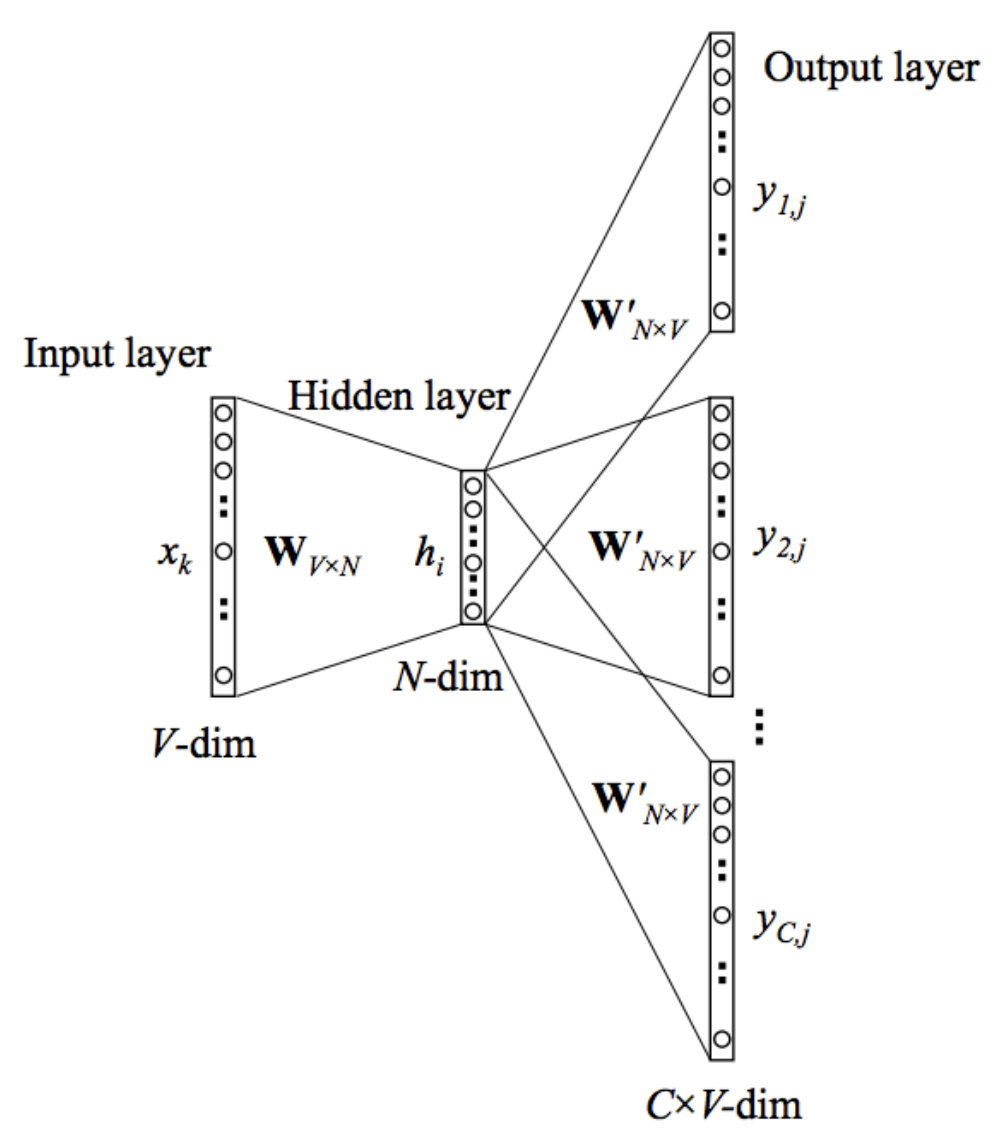
\includegraphics[scale=0.4]{skip-arch}
    \label{skip-arch}
\end{center}
Using some regularization and computationnal tricks during the training,
as replacing the softmax output function computation by a 
hierarchical softmax computation, or as using negative sampling loss
as an objective function, or doing frequency subsampling; which are 
detailed in \cite{Mikolov2013}; Word2Vec embeddings achieved better 
generalization and denoising properties than SVD. The main 
idea behind both Word2Vec and SVD embeddings, which makes them 
coherent as a good semantic representation, is called 
the distributionnal hypothesis. This linguistic hypothesis is built upon
Firth's statement that \textit{"a word is characterized by the 
company that it keeps"}. Thus, words employed in similar contexts
are more likely to have similar meanings. However, latest deep learning 
developments seem to have abandoned this approach, replaced by language modelling
as in \cite{howard2018universal, Peters_2018, devlin2018bert}, which 
are outside the scope of this project. \\ \\
The evaluation of such embeddings is difficult, as they are learned in an 
unsupervised way. However, two techniques are generally used to assess
embeddings representation quality : the evaluation of the embedding through
a downstream task, i.e. for instance the evaluation of classic text classifiers 
using the evaluated embedding as an input; and an evaluation through 
word similarities, with the objective that near vectors (regarding 
cosine distance) represent words with similar meanings. This evaluation
techniques are used in the same manner for text embeddings.

\subsection{From word embeddings to text embeddings}

In natural language processing, and more specifically in 
high-level tasks, there is no interest on studying single words. 
Thus, a natural question when working on texts, is : how to 
transform word embeddings to a single text embedding? In this section
we will describe 'natural' text embeddings, resembling the co-occurence
matrix described above, used in the article; and LSTMs embeddings, 
which are now more commonly used.

\subsubsection{Bag of n-Grams/Cooccurrences}

In this part, we will suppose that we have a vocabulary 
$\mathcal{V} = \{ v_1, ..., v_V\}$ and a document $d=w_1, ..., w_T$, 
where $w_i \in \mathcal{V}$ for any $i=1, ..., T$, and a fixed integer 
$n\in \N$. We recall 
that a $n$-gram is a sequence of $n$ words, 
for instance the set of unigrams is $\{v_1, ..., v_T \}$, the set 
of bigrams is $\{(v_1,v_2), (v_2, v_3), (v_1, v_3) ..., (v_{V-1}, v_V) \}$, etc.
We let $V_k$ be the number of possible $k$-grams over $\mathcal{V}$,
independently of order ($V_1 = V$), and 
$V_n^{\text{sum}} = \sum_{k=1}^n V_k$.\\ \\
For any $k\in \N$, let $B_k$ be a vector indicating, 
for any possible $k$-gram over $\mathcal{V}$, the number 
of occurences of this $k$-gram in the document.
A Bag-of-$n$-Grams, denoted $x^{\text{BonG}}$ is the concatenation of all the $B_k$ vectors
for $k = 1, ..., n$ : 
\[
x^{\text{BonG}} = [B_1, ..., B_N]\]
In order to simplify and get rid of order in the n-grams, author
merge the $k$-grams in the vocabulary that are the same words in a 
different order. Then, we can write :
$B^{\text{Co-oc}}_k = \sum_{t=1}^{T-k+1} e_{ \{w_t, ..., w_{t+k-1}\}  }$. 
A Bag-of-$n$-Co-occurrences (BonC) is then :

\[
x^{\text{BonC}} = [B^{\text{Co-oc}}_1, ..., B^{\text{Co-oc}}_N]\]

These embeddings are sparse, $V_n^{\text{sum}}$-dimensional vectors.


\subsubsection{DisC embeddings}
This document embeddings relies on word embeddings. 
Supposing that we have learned word embeddings and that we denote
$x_{v_i} \in \R^d, d<<V$ the embedding of the word $v_i \in \mathcal{V}$, for any
$i=1,..., n$; and that we still have our document $d= w_1, ..., w_T$; 
then the unigram embedding of the document is :
\[z^u = \sum_{t=1}^T x_{w_t}\]
$z^u$ can be re-written as the product of a compression matrix $A$ 
in which columns are word embeddings $x_w$; and the "Bag-of-1-grams" document embedding : 

\[z^u = Ax^{\text{Bo1G}} = \sum_{t=1}^T A e_{w_t} = \sum_{t=1}^T x_{w_t} \]
Authors extend this unigram definition to $n$-co-occurrences by using
element-wise multiplication of word embeddings, defining: 
\[\tilde{x}_{\{w_1, ..., w_n\}} = d^{(n-1)/2} \odot_{t=1}^n x_{w_t} \ \ \in \R^d \]
Then, DisC (distributed co-occurence) embeddings are defined as
the concatenation of:

\[
    z^{(n)} = \left [ 
                C_1 \sum_{t=1}^T \tilde{x}_{w_t}, 
                ..., 
                C_n \sum_{t=1}^{T-n+1} \tilde{x}_{\{w_t, ..., w_t+n-1\}}
              \right ]
              \in \R^{nd}
\]
With $C_1,..., C_n$ being scaling factors, detailed later. As in the 
unigram case, DisC embeddings are directly related to compressed sensing
as we can find $A^{(n)}\in R^{dn \times V_n^{\text{sum}}}$ such that:
\[z^{(n)} = A^{(n)}x^{BonC} \]

\subsubsection{LSTMs}

LSTMs, which stands for Long-Short-Term Memory are a kind of recurrent
neural networks (RNN), introduced in \cite{Hochreiter:1997:LSM:1246443.1246450}.
As with classic RNNs, the point in LSTMs is to be able to 
handle sequential data, say for instance a document made of already 
embedded words :

\[   x =\{x_1, ..., x_T \} \]

\noindent A given LSTM cell $A$ 'evolves' with the time, and is caracterized in time 
by a \textit{hidden state} $h_t$ and a \textit{memory} $c_t$. We denote $A^{(t)}$ the state of cell
$A$ at time $t$. $A^{(t)}$   has three inputs : 
\begin{itemize}
    \item $h_{t-1}$, the hidden state transmitted by the previous cell state $A^{(t-1)}$. 
    \item $c_{t-1}$, the memory transmitted by the previous cell state $A^{(t-1)}$.
    \item $x_t$, the 'real' sample input
\end{itemize}
And two outputs : 
\begin{itemize}
    \item $h_{t}$, the updated hidden state transmitted to  $A^{(t+1)}$. 
    \item $c_{t}$, the updated memory transmitted to  $A^{(t+1)}$.
\end{itemize}
These inputs and outputs are schematized in Figure \ref{fig:LSTM1} \footnote{The figure is extracted from Christopher Olah's excellent blog : \href{http://colah.github.io/posts/2015-08-Understanding-LSTMs/}{http://colah.github.io/}}. 
The core question of LSTMs is to define update rules for $h_t$ and $c_t$. First, we want to 
know how to update memory, or in other words, which informations to forget and which informations
to remember. To do so, we define :
\begin{itemize}
    \item $i_t = \sigma\left ( x_t U^i + h_{t-1} X^{i}\right) \in [0, 1]$, where $U^i, W^i$ are weights to learn.
         This function is called the \textit{input gate}. The input gate is a weighted sum of
         the sample data at time $t$ and the previous hidden state of the cell, regularized by the sigmoid function.
         The inpute gate decides, what new information we are going to store in the updated memory, and in
         which proportion, depending on the precedent data. 
    \item $\tilde{c}_t = \tanh \left ( x_t U^c + h_{t-1} X^{c}\right ) \in [-1, 1] $, where $U^c, W^c$ are weights to learn.
    $\tilde{c}_t$ is a candidate for creating 'new $c_{t}$ values'.
    \item $f_t = \sigma \left (x_t U^f + h_{t-1} X^{f}\right ) \in [0,1]$, where $U^f, W^f$ are weights to learn.
    This is called the \textit{forget gate}. The forget gate decides the proportion at which each element of the 
    memory is going to be forgotten.
\end{itemize}

\noindent The memory can then be updated, with respect to the following rule:
\begin{align*}
    c_t = f_t * c_{t-1} + i_t * \tilde{c}_t
\end{align*}

\noindent Finally, to update the hidden state, we define the \textit{output gate} in the same fashion, and we update $h_t$ :

\begin{align*}
    o_t &= \sigma \left (x_t U^o + h_{t-1} X^{o}\right ) &\in& [0,1]  \\
    h_t &= \tanh (c_t) * o_t  &\in& [-1, 1]
\end{align*}




Some variants of LSTM cells may define input, output and forget gates differently. For instance,
the peephole version of LSTM implements the natural idea that the previous memory state $c_{t-1}$
has to be considered when deciding the input, output and forget rates.  GRU, Gated Recurrent Units 
are other variants of LSTMs. \\ \par 

\begin{center}
    \captionof{figure}{A representation of a LSTM cell in time}
    \label{fig:LSTM1}
    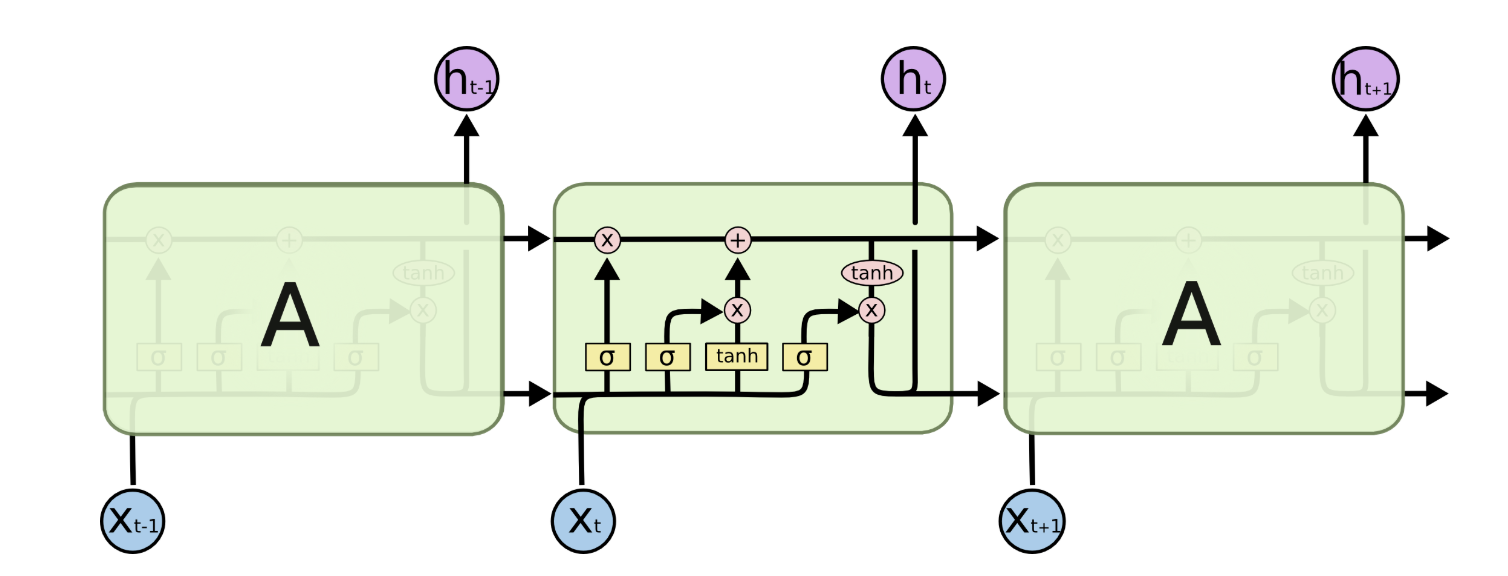
\includegraphics[scale=0.3]{LSTM.png}
\end{center}
One question remains : what exactly is the hidden state $h$? 
$(h_t)_{t=1...T}$ can be viewed as the 'output' of the LSTM.  
In our case, the final hidden state $h_T$ is directly used as 
the document embedding. This representation of the document 
is unsupervised, and the LSTM is usually trained on another 
task, regarding which $(h_t)_{t=1...T}$ are features (see for 
instance \cite{Lample_2016} for an example of LSTMs trained 
for named entity recognition). 

Appart from having a very flexible and modular structure,
 LSTMs cells do not suffer of the same 
vanishing gradient problem as RNNs in practice,
 and are thus more effective
in modelling sequential data. They are particularly adapted 
to NLP problems because of their 
sequential nature. 


% \subsection{Why text embeddings? }


% Now that we have presented text embedding, we can present some of 
% their most well-known applications. As text embeddings 
% are a general, abstract, numerical representation for texts, 
% they serve in many NLP tasks : text classification, and 
% more specifically sentiment analysis (is a product review positive, 
% negative, or neutral?), text similarity analysis, but 
% also information retrieval. In information retrieval (IR), 
% a common problem is to find the most relevant documents 
% regarding a query. In classic IR systems, documents are compared 
% with queries through co-occurence matrices, or through TF-IDF, 
% which is commonly used in tech as it i a central part in 
% Lucene and ElasticSearch algorithms. However, modern IR 
% systems focuss on finding document and queries embeddings, 
% in order to match the two by comparing them in a common 
% latent space. Thus, text embeddings are useful in many 
% machine learning tasks, but also in information retrieval 
% problems. 

% \newpage
\section{Learning to classify in the compressed domain}

Texts can be viewed as a collection of sparses measures (words) 
over a complex signal (ideas, a meaning, a sentiment, etc.). The
text embedding problem is thus directly a compressed sensing problem : 
using a compression (=embedding) matrix $A$ over a collection of 
words $x=w_1, ...w_T$ to produce a dense, compressed representation 
$z = Ax$, with good reconstruction qualities. As the "reconstruction"
quality of the compressed signal cannot, in this case, 
be properly evaluated, we need results on this reconstruction
quality through a downstream task as classification. 

\subsection{Results on compressed sensing for classification}

As we are interested in the evaluation of text embeddings through 
text classification, the compressed learning approach proposed 
in \cite{Calderbank2009CompressedL} (generalized and modified in 
our article of interest \cite{arora2018sensing}) gives us a useful result
stated in \ref{th1}. This result tells us how training a linear 
classifier over the compressed data instead of the original data 
penalizes the classification results. \\ \\We chose to reproduce the
 ideas of proof of this theorem here, with more detail in general, as we think that it is 
an very interesting result regarding the compressed sensing course. 

\begin{theorem}\label{th1}
    For any subset $\mathcal{X}\subset \R^N$ containing the origin, 
    let $A\in \R^{d\times N}$ be $(\Delta \mathcal{X}, \varepsilon)-$RIP, and $m$ 
    samples $S=\{ (x_i, y_i)\} \subset \mathcal{X}\times \{-1, 1\}$
    be drawn i.i.d. from the same distribution $\mathcal{D}$ over 
    $\mathcal{X}$, with $||x||_2 \leq R$. \\ 
    If $l$ is a $\lambda$-Lipschitz convex loss function and $w_0\in \R^N$
    is its minimizer over $\mathcal{D}$, then, with probability
    $1-2\delta$, the linear classifier $\hat{w}_A\in \R^d$ minimizing the 
    $l_2$-regularized empirical loss function $l_{S_A}(w)+\frac{1}{2C} ||w||_2^2$
    over the compressed sample $S_A = \{(Ax_i, y_i) \}_{i=1}^m
    \subset \R^d \times \{-1, 1\} $ satisfies :
    \begin{align}
        l_{\mathcal{D}}(\hat{w}_A) &\leq 
        l_{\mathcal{D}}(w_0) + \mathcal{O}
        \left ( 
            \lambda R ||w_0||_2 \sqrt{\varepsilon + \frac{1}{m}\log\frac{1}{\delta}}
        \right )
    \end{align}
    for an appropriate choice of $C$, and recalling that
     $\Delta \mathcal{X} = \{x-x' : x, x' \in \mathcal{X} \}$, for 
     any $\mathcal{X}\subset \R^N$
\end{theorem}

    As the proof is a bit complex, we are going to explain its outline first.
    The idea is to first define an empirical (regularized) risk minimizer on both 
    the sparse and the compressed domain, respectively $\hat{w}, \hat{w_A}$.\\ 
    In parallel, we define the theoretical (regularized) risk minimizer 
    (which minimizes the loss expectation over the 
    whole distribution $\mathcal{D}$ ), also both in the sparse 
    and in the compressed domain, respectively $w^*, w_A^*$. \\
    On the compressed domain, we compare the loss of $\hat{w_A}$ with 
    the loss of $w_A^*$. Using a lemma deduced from the RIP condition over $A$
    and a result from \cite{NIPS2008_3400}, we compare the 
    losses of $w_A^*$ and $A\hat{w}$. The same lemma enables us to 
    compare the losses of $A\hat{w}$ and $\hat{w}$. Finally, 
    we compare the losses of $\hat{w}$ and $w^*$. \\ \\

    First define the $l_2$-regularization of the loss function $l$ as :
    \[L(w) = l(w) + \frac{1}{2C}||w||_2^2\]

    \begin{lemma} \label{lemma1}
        Let $\hat{w}$ be the classifier obtained minimizing :
        $L_S(w) = \frac{1}{m} \sum_{i=1}^m l(w^Tx_i, y_i) + \frac{1}{2C}||w||_2^2 $,
        i.e. $\hat{w}$ is the empirical (regularized) risk minimizer,
        where $l(., .)$ is a convex $\lambda$-Lipschitz function in the first coordinate. 
        Then :
        \[\hat{w} = \sum_{i=1}^m \alpha_i y_i x_i , \ \ \
        |\alpha_i|\leq \frac{\lambda C}{m}, \forall i\]
        The result holds in the compressed domain.
    \end{lemma}
    \begin{proof}
         By convexity, the only optimizer can be found
        by taking first-order conditions :
        \begin{align*}
            \partial_w L_S(w) &= 
                    \frac{w}{C} + \frac{1}{m} \sum_{i=1}^m \partial_{w^Tx_i} l(w^T x_i, y_i)x_i
        \end{align*}
        Then, we have :
        \begin{align*}
            \hat{w} &=- \frac{C}{m} \sum_{i=1}^m \partial_{\hat{w}^Tx_i} l(\hat{w}^T x_i, y_i)x_i \\
                    &= \frac{C}{m} \sum_{i=1}^m - y_i\partial_{\hat{w}^Tx_i} l(\hat{w}^T x_i, y_i) y_i x_i
        \end{align*}
        As $y_i\in \{-1, 1\}$. 
        $l$ is a $\lambda$-Lipschitz function, thus its sub-gradient 
        is bounded by $\lambda$, implying $|\partial_{\hat{w}^Tx_i} l(\hat{w}^T x_i, y_i)| \leq \lambda$. 
        Hence the result.
    \end{proof}
    \begin{lemma}\label{lemma2}
        \[ x, x' \in \mathcal{X} 
        \Rightarrow 
        (1+\varepsilon) x^Tx' - 2R^2 \varepsilon 
        \leq (Ax)^T (Ax') 
        \leq (1-\varepsilon) x^Tx' + 2R^2 \varepsilon 
        \]
    \end{lemma}
    \begin{proof}
        In one of our hypothesis, $A$ is $(\Delta \mathcal{X}, \varepsilon)$-RIP. 
        Then, by definition : 

        \begin{align*}
            (1-\varepsilon) ||x-x'||_2 
            \leq ||A(x-x')||_2
            \leq (1+\varepsilon) ||x-x'||_2 
        \end{align*}
        % Using the fact that if $x, x'$ are $k$-sparse, then $x-x'$ is 
        % $2k$:-sparse
        Using this, we show the first side of the inequation, 
        as the other side is symmetric :
        \begin{align*}
            ||A(x-x')||_2^2 &= ||Ax||^2_2  + ||Ax'||^2_2 - 2 (Ax)^T(Ax') \\
            (1-\varepsilon) ||x-x'||^2_2 &\leq ||Ax||^2_2  + ||Ax'||^2_2 - 2 (Ax)^T(Ax') \\
            (1-\varepsilon) (||x||^2_2+||x'||^2_2 -2x^T x') 
            &\leq ||Ax||^2_2  + ||Ax'||^2_2 - 2 (Ax)^T(Ax') \\
        \end{align*}
        As $0_N \in \mathcal{X}$, $A$ is also $(\mathcal{X},
         \varepsilon)$-RIP, leading to having :
        $||Ax||^2_2 \leq (1+\varepsilon)||x||^2_2$, and thus :
        \begin{align*}
            (1-\varepsilon) (||x||^2_2+||x'||^2_2 -2x^T x') 
            &\leq (1+\varepsilon)(||x||^2_2  + ||x'||^2_2) - 2 (Ax)^T(Ax') \\
        \end{align*}
        Finally, using the hypothesis : $||x||_2 \leq R$, 
        \[  (Ax)^T(Ax') \leq (1-\varepsilon)x^Tx' + 2R^2\varepsilon \]
    \end{proof}
    \begin{corollary}
        \[
            ||\hat{w}||_2^2 
            \leq \lambda^2 C^2 R^2 \text{ and }
            ||\hat{w}_A||_2^2 
            \leq \lambda^2 C^2 (1+\varepsilon)^2 R^2
        \]
    \end{corollary}
    \begin{proof} \label{corollary1}
        Using \ref{lemma1} when calculating $||\hat{w}||_2^2$, and using
        $||x||_2\leq R$, we find the first bound. Using \ref{lemma2}, when 
        calculating $||\hat{w}_A||_2^2$, and $||x||_2\leq R$, we find the 
        second bound.
    \end{proof}
    \begin{lemma}\label{lemma3}
        \begin{align*}
             L_{\mathcal{D}} (A\hat{w}) \leq 
             L_{\mathcal{D}}(\hat{w}) + \mathcal{O}(\lambda^2 C R^2 \varepsilon)
        \end{align*}
    \end{lemma}
    \begin{proof}
        As this proof is very focused on calculations, we will only insist on 
        most important points, and not whole computations. \\ \\
        First, we use \ref{lemma1} to have that :
        \begin{align*}
            (A\hat{w})^T(Ax)  = \sum_{i=1}^m \alpha_i y_i (A x_i)^T(Ax)
        \end{align*}
        Using \ref{lemma2}, 
        \begin{align*}
            \hat{w}^Tx - 3\lambda CR^2\varepsilon 
            \leq (A\hat{w})^T(Ax) 
            \leq \hat{w}^Tx + 3\lambda CR^2\varepsilon 
        \end{align*}
        As $l$ is $\lambda$-Lipschitz, we can take the expectations over $\mathcal{D}$:
        \begin{align} \label{loss1}
            l_{\mathcal{D}}(A \hat{w}) \leq l_{\mathcal{D}}(\hat{w}) +  3\lambda CR^2\varepsilon
        \end{align}
        We now want to compute $||A\hat{w}||_2^2 $:
        \begin{align*}
            ||A\hat{w}||_2^2  &= 
                (A\hat{w})^T(A\hat{w}) \\
                &=(\sum_{i=1}^T\alpha_i y_i x_i)^T
                (\sum_{j=1}^T\alpha_j y_j x_j) \\
                &= \sum_{i=1}^T \sum_{j=1}^T 
                \alpha_i \alpha_j  
                y_i y_j
                (Ax_i)^T (Ax_j) \\
        \end{align*}
        Using \ref{lemma2}, 
        \begin{align*}
            ||A\hat{w}||_2^2  &\leq ||\hat{w}||_2^2 + 3 \lambda^2 C^2 R^2 \varepsilon \\
            \Leftrightarrow \frac{1}{2C}||A\hat{w}||_2^2  &\leq\frac{1}{2C} ||\hat{w}||_2^2 + \frac{3}{2} \lambda^2 C R^2 \varepsilon 
        \end{align*}
        With this inequality and using \ref{loss1}, we have the result.
    \end{proof}
    We have shown some results on $\hat{w}$, the empirical regularized
    risk ($L_S$) minizer. We are now interested in $w^*$, the theoretical regularized
    risk ($L_\mathcal{D}$) minimizer. 
    \begin{lemma} \label{lemma4}
        Letting $w^*$ be the linear classifier minimizing 
        $L_\mathcal{D}$, we have that, with probability $1-\gamma$ : 
        \begin{align*}
            L_\mathcal{D}(\hat{w}) 
            &\leq L_\mathcal{D}(w^*) 
            + \mathcal{O}\left (\frac{\lambda^2 C R^2}{m}\log \frac{1}{\gamma} \right )
        \end{align*}
    This result holds in the compressed domain.
    \end{lemma}
    \begin{proof}
        Corollary \ref{corollary1} tells us that :
        \[
            ||\hat{w}||_2^2 
            \leq \lambda^2 C^2 R^2 \text{ and }
            ||\hat{w}_A||_2^2 
            \leq \lambda^2 C^2 (1+\varepsilon)^2 R^2
        \]
        In other words, $\hat{w}$ and $\hat{w_A}$ are contained 
        in a closed convex subset independent of $S$. Authors use the 
        fact that $l$ is $\lambda$-Lipschitz to say that $L$ is strongly 
        $\frac{1}{C}$-strongly convex. Moreover, $||x||_2 \leq R$. 
        A theorem in \cite{NIPS2008_3400} can be applied, giving that
        with probability $1-\gamma$:
        \begin{align*}
            L_{\mathcal{D}}(\hat{w}) - L_{\mathcal{D}}(w^*) 
            \leq 2 [L_{\mathcal{S}}(\hat{w}) - L_{\mathcal{S}}(w^*)]_+ 
            + \mathcal{O}\left( \frac{\lambda^2C R^2}{m} \log \frac{1}{\gamma}  \right)
        \end{align*} 
        By definition, $\hat{w}$ minimizes $L_S$, thus :
        $[L_{\mathcal{S}}(\hat{w}) - L_{\mathcal{S}}(w^*)]_+  = 0$, and the result follows 
        directly. 
    \end{proof}
\noindent \textbf{Proof of the theorem}:
\begin{proof} As 
$l_{\mathcal{D}}(\hat{w}_A) \leq l_{\mathcal{D}}(\hat{w}_A) 
+ \frac{1}{2C} ||w^*_A||_2^2 = L_{\mathcal{D}(\hat{w_A})}$.
Lemma \ref{lemma4}, applied to the compressed domain gives :
\[ l_\mathcal{D}(\hat{w_A}) \leq
    L_\mathcal{D}(\hat{w_A}) 
    \leq L_\mathcal{D}(w_A^*) 
    + \mathcal{O}\left (\frac{\lambda^2 C R^2}{m}\log \frac{1}{\gamma} \right )
\]
As $w^*_A$ is the minimizer of
 $L_{\mathcal{D}}, L_{\mathcal{D}}(w*_A) \leq L_{\mathcal{D}}(A\hat{w}) $.
Thus 
\begin{align*}
    l_\mathcal{D}(\hat{w_A}) 
    &\leq L_\mathcal{D}(A\hat{w}) 
    + \mathcal{O}\left (\frac{\lambda^2 C R^2}{m}\log \frac{1}{\gamma} \right ) \\
    &\leq L_\mathcal{D}(\hat{w}) + \mathcal{O}(\lambda^2 C R^2 \varepsilon)
    + \mathcal{O}\left (\frac{\lambda^2 C R^2}{m}\log \frac{1}{\gamma} \right ) 
    \text{    (lemma 2.5)}\\
    &\leq L_\mathcal{D}(\hat{w}) 
    + \mathcal{O}\left ( 
        \lambda^2CR^2 \left (
        \varepsilon + \frac{1}{m} \log(\frac{1}{\gamma})
        \right ) \right ) \\
\end{align*}
In the sparse domain, lemma \ref{lemma4} assure that : 
$L_{\mathcal{D}}(\hat{w}) \leq L_{\mathcal{D}}(w^*) + \mathcal{O}\left (\frac{\lambda^2 C R^2}{m}\log \frac{1}{\gamma} \right )
$.
We put this inequality in the last inequality to have:
\begin{align*}
    l_\mathcal{D}(\hat{w_A})    
    &\leq L_\mathcal{D}(w^*) 
    + \mathcal{O}\left ( 
        \lambda^2CR^2 \left (
        \varepsilon + \frac{1}{m} \log(\frac{1}{\gamma})
        \right ) \right )
\end{align*}
Finally, as $w^*$ minimizes $L_{\mathcal{D}}$, 
$L_{\mathcal{D}}(w^*) \leq L_{\mathcal{D}}(w_0) =
 l_{\mathcal{D}}(w_0) + \frac{1}{2C}||w_0||_2^2$
 Which leads to:
 \begin{align*}
    l_\mathcal{D}(\hat{w_A})    
    &\leq  l_{\mathcal{D}}(w_0) + \frac{1}{2C}||w_0||_2^2
    + \mathcal{O}\left ( 
        \lambda^2CR^2 \left (
        \varepsilon + \frac{1}{m} \log(\frac{1}{\gamma})
        \right ) \right )
 \end{align*}
 The theorem follows easily by optimizing $C$. 
\end{proof}


\subsection{Application on LSTMs}



% \section{Sparse recovery from text embeddings}

% \subsection{Random word embeddings}

% \subsection{Pretrained word embeddings}





% \newpage
% \section{Experiments and discussion}

% \subsection{Results reproduction}

% \subsection{Testing DisC embeddings on real life data}


% \subsection{Discussion}


\newpage 
\pagenumbering{gobble}
\bibliography{references} 
\bibliographystyle{ieeetr}
\end{document}